%&pdflatex
%% filename: amsart-template.tex, version: 2.1
\documentclass[reqno]{amsart}

\usepackage{hyperref}
\usepackage{inputenc}
\usepackage{graphicx}
\usepackage{bbm}
\usepackage{amssymb}
\usepackage{listings}
\usepackage{float}


% \newtheorem{theorem}{Theorem}[section]
% \newtheorem{lemma}[theorem]{Lemma}
% \theoremstyle{definition}
% \newtheorem{definition}[theorem]{Definition}
% \newtheorem{example}[theorem]{Example}
% \newtheorem{xca}[theorem]{Exercise}
% \theoremstyle{remark}
% \newtheorem{remark}[theorem]{Remark}
% \numberwithin{equation}{section}
% \setlength{\parindent}{0pt} % turn off auto-indent

% \graphicspath{ {./} }

\begin{document}

\title{Kaggle competition: drawing classification}

\author{L\'ea Ricard, Jeff Sylvestre Decary \& Joseph D. Viviano}

\address{Universit\'e de Montr\'eal}
\curraddr{}
\email{lea.ricard@umontreal.ca, jeff.sylvestre-decary@polymtl.ca, joseph@viviano.ca}
\thanks{}
\date{Nov 2018}

\maketitle

\noindent 
Team: Madame Ricard and the Booster Boyz: L\'ea Ricard (20085993), Jeff Sylvestre Decary (20121588) and Joseph D. Viviano (20115694).



\section{Introduction}
% Very briefly describe the problem and summarize your approach and results.
Our task was to build a classifier capable of categorizing hand-drawn images into 31 categories. We were provided with a variant of Google's \textit{Quick draw!} dataset \cite{Quick_draw}. The images consisted of a drawing positioned randomly on a white canvas, with added random noise around the drawing. The training set contains 10 000 labeled images with $100\times100$ pixels and the test set contains 10 000 unlabeled images with the same numbers of pixels. The proportion of each class in the training set differs from class to class, going from 1.6\% (squid) to 5.7\% (mouth) (see Appendix \ref{data}). The empty class contains no drawing and only random noise.
\section{Feature design}
% Describe and justify any pre-processing methods, or how you designed and selected your features
The images are pre-processed differently for scikit-learn models than for pytorch models as we utilized data-augmentation for the resnet mode. For the scikit learn models, we simply scaled the data into the range $[0, 1]$, and stored the data as a $n \times m$ matrix (number of samples, number of pixels per image). For the pytorch models, the data was stored in a $n \times w \times h$ tensor (number of samples, image width, image height). These images were also normalized into a range of $[0, 1]$. For data augmentation, each image was randomly flipped horizontally and vertically per batch, and Gaussian noise was added pixel-wise with a mean of 0 and sigma=0.1. The outputs of this were again clipped to the range of $[0, 1]$.\\

Raw images (figure \ref{fig:cropping} (a)) are also cropped using a process of (figure \ref{fig:cropping} (b)) denoising with a median filter, (figure \ref{fig:cropping} (c)) segmenting by edge detection, (figure \ref{fig:cropping} (d)) cropping the biggest connected component on the raw image and (figure \ref{fig:cropping} (e)) patching to a standard size of $40 \times 40$ pixels. This preprocessing was not used in the ResNet convolutional neural netowrk final model, as discussed in section \ref{Discussion}.\\

\begin{figure} [H]
\centering
\begin{tabular}{cccc}
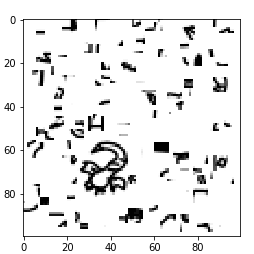
\includegraphics[width=0.25\textwidth]{Figures/raw.png} &
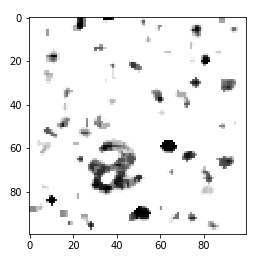
\includegraphics[width=0.25\textwidth]{Figures/denoised.png} &
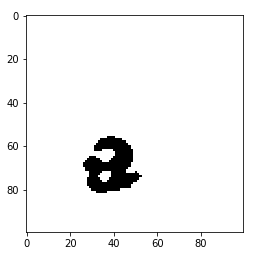
\includegraphics[width=0.25\textwidth]{Figures/biggest_connected_element.png} \\
(a)  & (b) & (c)  \\[6pt]
\end{tabular}
\begin{tabular}{cccc}
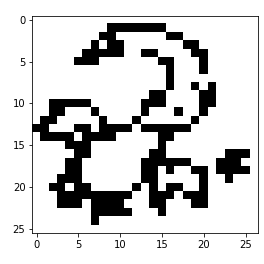
\includegraphics[width=0.25\textwidth]{Figures/crop.png} &
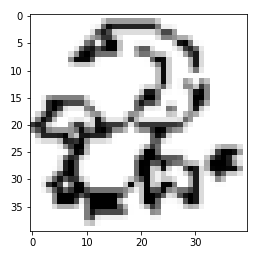
\includegraphics[width=0.25\textwidth]{Figures/crop_standardize.png} \\
(d)  & (e)  \\[6pt]
\end{tabular}
\caption{(a) raw
(b) denoised
(c) biggest connected component
(d) cropped
(e) patched
image}
\label{fig:cropping}
\end{figure}

\section{Algorithms}
% Give an overview of the learning algorithms used without going into too much detail.
We used scikit learn to build baseline logistic regression and linear SVM models. They performed poorly, so attempted higher capacity models such as kernelized SVM, k-nn, and convolutionnal neural networks. More specifically, we used Residual neural network (ResNet) models with 18 and 101 layers, respectively.\\

We were expecting that the ResNet model would outperform the other models since convolutional neural networks tend to perform best for object detection tasks. The unique aspect of ResNets is that they have skip connections that allow deeper layer of the network to have direct access to the activations of earlier layers \cite{He}.

\section{Methodology}
% Include any decisions about training/validation split, distribution choice for naive bayes, regularization strategy, any optimization tricks, setting hyper-parameters, etc.

We started by splitting our initial training set into a training ($n=9000$) and a validation set ($n=1000$). For all scikit-learn models, we used the training set to learn the parameters of the model and the validation set to do hyperparameter selection using randomized search \cite{Berg} with 25 iterations, and 3 fold inner-loop cross validation (these folds were applied to the training data only). This procedure was performed in the context of outer 5-fold stratified cross validation to find the model with the best average accuracy across all folds. Empirical risk was estimated at the end of training by generating predictions with the best model on the test set.\\    

For the ResNet model, began with a model available in torchvision, which we then fine tuned. We used Stochastic Gradient Descent(SGD) with momentum and weight decay to learn the weights. We did a small grid search over the following hyperparameters: number of layers (18 or 101), momentum (0.65, 0.9, 0.95), learning rate ($10^{-3}$, $10^{-4}$, $10^{-5}$), and weight decay ($10^{-3}$, $10^{-4}$, $10^{-5}$, $10^{-6}$, $10^{-8}$). We trained each model for 100 epochs with early stopping and a patience of 25 epochs (i.e, we stopped training if we do not beat the best accuracy after 25 epochs). For almost all models, the best model was found around epoch 50, except when weight decay was very strong and the model tended not to achieve good performance. We used a minibatch size of 32 for all models. the final model selected via early stopping was used to estimate the empirical risk with via predictions on the test set.\\

\begin{figure}
    \centering
    \begin{subfigure}
        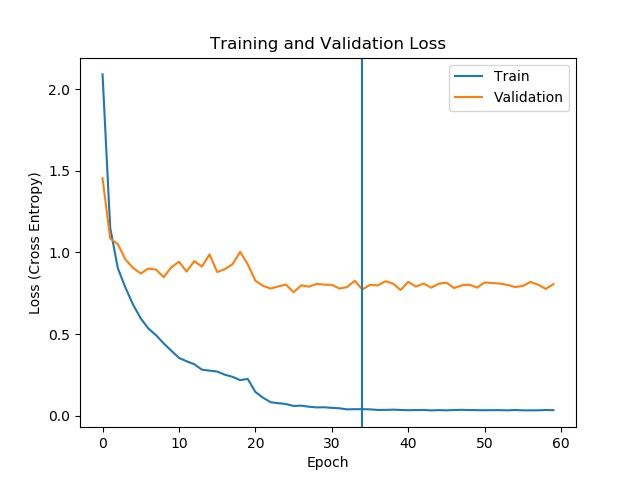
\includegraphics[width=.4\linewidth]{Figures/training_loss.jpg}
    \end{subfigure}
    \begin{subfigure}
        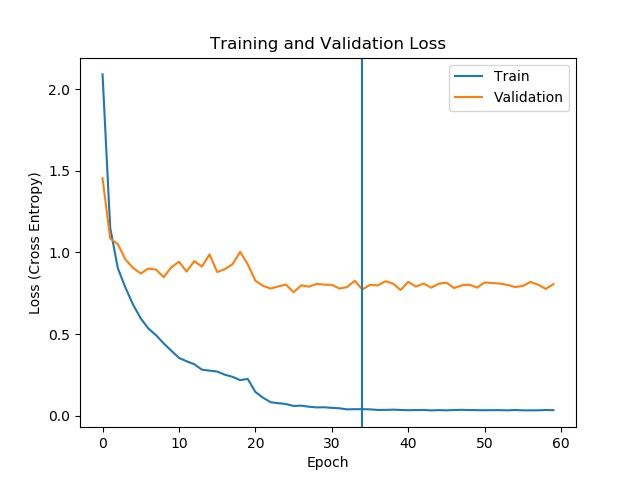
\includegraphics[width=.4\linewidth]{Figures/training_loss.jpg}
    \end{subfigure}
    \caption{Loss and Performance Learning Curves for ResNet Model}
    \label{fig:my_label}
\end{figure}

\section{Results}
% Present your results, with emphasis on i) one simple baseline and ii) on the method that gave you the best performance. You do not need to show the results from all methods that you tried.

The accuracy of the image classification on the training set, the validation set and the test set of the different models are shown in table \ref{fig:results}. The ResNet far outperformed the other models, both on the validation set and on the test set. We can see from the accuracy on the training set that logistic regression and linear SVM models, our baseline, did not have sufficient capacity for the task. \\

The confusion matrix of the logistic regression (Appendix \ref{confusion}) shows that certain labels are never predicted (ex. parrot, peanut), when others (ex. mouth, pineapple) are predicted too often. By comparing with the training set distribution table (Appendix \ref{data}), we see that those never predicted are less common in the training set. Therefore these low capacity models focused on predicting the most likely classes. The performance of the SVM model increases significantly when we allow the use of non-linear kernels. The ResNet achieved 82.1\% accuracy on the test set.

\begin{table}
\caption {Accuracy of models} \label{fig:results}
\begin{center}
\begin{tabular}{|l|l|l|l|l|}
    \hline
    &&\multicolumn{3}{|c|}{Accuracy (\%)}\\
    \hline
    Model & Library & Training set & Validation set & Test set\\
    \hline \hline
     LR & sklearn & 34.2 & 31.3 & 14.0\\
     Linear SVM & sklearn & 46.6 & 25.20 & 12.5 \\
     Kernelized SVM & sklearn & 64.4 & 41.8 & 18.6 \\
     %GBM &  &  &  & \\
     KNN & sklearn & 42.9 & 27.6 & - \\
     %Xgb & Xgboost &99.3  &20.2  &11.9 \\
     ResNet & pytorch & 99.5 & 82.5 & 82.1 \\
     \hline
\end{tabular}
\end{center}
\end{table}

\section{Discussion}
% Discuss why your best method performs better than the simple baseline. Which design choices where the most impactful on performance?
\label{Discussion}

Pre-processing the images by cropping them was crucial for lower capacity models. The accuracy of baseline models trained on raw images was close to chance, because those models only make pixel-wise comparisons. Hence, if we ask a SVM to compare two similar drawings placed in different corners of a white canvas, the model cannot associate similarities present across locations in space. Cropping partially resolved this issue by putting all drawings in roughly the same location. The ResNet did not benefit from this, as convolutional models can learn to detect features at (roughly) any location on the input images. In practice, using crops as a preprocessing step for the ResNet led to slighly worse performance for the best-performing model (80.5\% vs 82.1\%), likely because the cropping procedure removed some useful information for some small proportion of the classes. For example, the cropping of an image with label 'empty' would be improper because it enlarges the largest sample of random noise in the image.
\\

Our first implementation of CNN was a ResNet with 18 layers including padding and stride in each layer. This model gave us a first score of 75.9\% on the test set. When we replaced the 18 layers model with a 101 layers model, out final score increased to  82.1\%. The best hyperparameters for this run were: momentum=0.9, learning rate=$10^{-4}$, and weight decay=$10^{-3}$. Interestingly, the optimal weight decay for the 18 layer network was much smaller at $10^{-5}$, because the model had less overall capacity and was not as prone to over-fitting to the training set. A cursory examination of the confusion matrix (Appendix \ref{confusion}) suggests the ResNet did not make more mistakes on any classes in particular. \\

For a given number of parameters, neural networks increase capacity as we increase the number of layers\cite{DL}, but are harder to train due to vanishing gradients. ResNets get around this using "shortcut connections", making it possible for deep layers to see a linear mixture of the activations of all previous layers during optimization \cite{He}. The use of deeper networks improved performance, as evidenced by the jump in accuracy between the 18 layer and 101 layer network. Data augmentation allowed us to train the model on a larger training set than provided, which is very likely to have helped generalization. We believe training was relatively quick for our models as we used transfer learning and models pre-trained on imagenet. Given more time and resources, we would have like to explore more forms of data augmentation (e.g., cropping, rotations), the use of even deeper networks, and the application of dropout to regularize our model. \\

%ADD: discussion about the distribution of the dataset


\section{Statement of contributions}
%Briefly describe the contributions of each team member towards each of the components of the project (e.g. defining the problem, developing the methodology, coding the solution, performing the data analysis, writing the report, etc.) At the end of the Statement of Contributions, add the following statement: We hereby state that all the work presented in this report is that of the authors.

The problem definition and the report writing has been done by all the team. Joseph developed the methodology and coded the ResNet model. L\'ea coded the baseline models, the knn and the kernelized SVM. She coded the cropping function as well. Jeff coded the gradient boosting machine and the extreme gradient boosting. We hereby state that all the work presented in this report is that of the authors.\\

\newpage
\begin{thebibliography}{99}
\bibitem{He} He, K., Zhang, X., Ren, S., & Sun, J. (2016). Deep Residual Learning for Image Recognition. 2016 IEEE Conference on Computer Vision and Pattern Recognition (CVPR), 770-778.\\

\bibitem{Quick_draw} Google, Inc. (2017). Quick Draw Dataset. Available from Quick Draw website: https://quickdraw.withgoogle.com/data\\

\bibitem{DL} Goodfellow, I., Bengio, Y., Courville, A., & Bengio, Y. (2016). Deep learning (Vol. 1). Cambridge: MIT press.\\

\bibitem{Berg} Bergstra, J., & Bengio, Y. (2012). Random search for hyper-parameter optimization. Journal of Machine Learning Research, 13(Feb), 281-305.

\end{thebibliography}


\appendix
\newpage
\section{Confusion matrices}
\label{confusion}
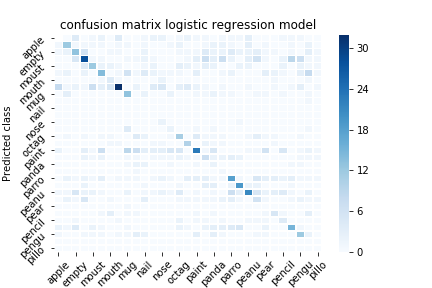
\includegraphics{Figures/confusion_lr_2.png}

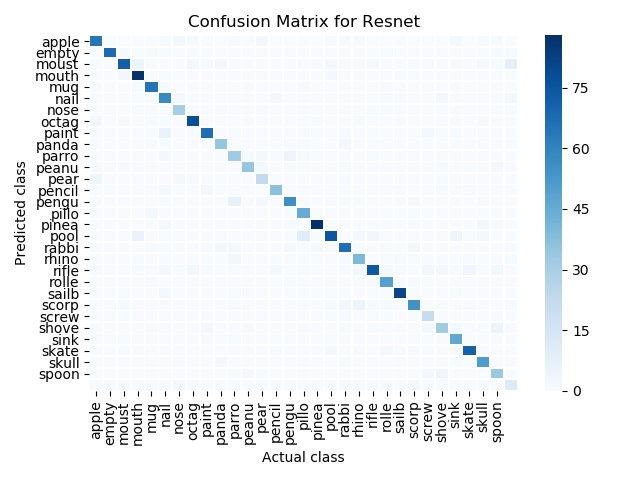
\includegraphics{Figures/resnet_confusionmat.jpg}

\newpage
\section{Data distribution}
\label{data}


\begin{table}[htp]
\caption {Training set distribution} \label{fig:data}
\begin{center}
\begin{tabular}{|l|l|l|}
    \hline
    Class label & Instances & \% \\
    \hline
    apple & 368	& 3.68\\
    empty &	323 & 3.23\\
    moust & 463	& 4.63\\
    mouth &	571 & 5.71\\
    mug & 382 & 3.82\\
    nail & 410 & 4.10\\
    nose & 204 & 2.04\\
    octag & 468 & 4.68\\
    paint & 314 & 3.14\\
    panda & 211 & 2.11\\
    parro & 206 & 2.06\\
    peanu & 199 & 1.99\\
    pear & 188 & 1.88\\
    pencil & 252 & 2.52\\
    pengu & 321 & 3.21\\
    pillo & 268 & 2.68\\
    pinea & 481 & 4.81\\
    pool & 479 & 4.79\\
    rabbi & 369 & 3.69\\
    rhino & 220 & 2.20\\
    rifle & 440 & 4.40\\
    rolle & 293 & 2.93\\
    sailb & 422 & 4.22\\
    scorp & 376 & 3.76\\
    screw & 182 & 1.82\\
    shove & 264 & 2.64\\
    sink & 272 & 2.72\\
    skate & 420 & 4.20\\
    skull & 288 & 2.8\\
    spoon & 182 & 1.82\\
    squig & 164 & 1.64\\
     \hline
\end{tabular}
\end{center}
\end{table}


\end{document}